\chapter{Evaluation and discussion}

Because SimGrid has already been thoroughly tested and validated, we do not
need to run extensive experiments to validate Batkube simulation models.
Moreover, since we only consider simple delay jobs, validation is not really
necessary. Still, even though the underlying models are sound, Batkube adds a
considerable overhead to Batsim because of the time synchronization between the
simulator and the scheduler. We want to verify to what extent time manipulation
impacts the scheduler behavior, and also that Batkube's fake Kubernetes API
mimics the real API well enough to let the scheduler run as expected. We then
conducted some validation experiments with simple workloads to verify that the
scheduler was correctly making its decisions.

In the next sections, we present the workloads and platforms we chose to study,
how we conducted experiments on a real cluster, and a study on Batkube's
parameters and their effect on the outputs.

\section{Experiments environment}

The entirety of the experiments are done with the default Kubernetes scheduler
\textbf{kube-scheduler} release \textbf{v1.19.0.rc-4} (commit 382107e6c84).
This choice was made because it is the standard choice for Kubernetes and
therefore the most commonly used scheduler in the industry, and because
supporting another scheduler would mean more development time which we did not
have. Still, it allowed us to conduct experiments to verify that the scheduler
behavior was not altered by Batkube.  All scripts used to run the experiment,
process the workloads and generate the graphs present in this report -- along
with some results -- are available on
\textit{batkube-test}\footnote{github.com/oar-team/batkube-test} repository.

\subsection{Real experimental testbed}

In order to validate the simulator results we then need to compare it against
workloads run on a real cluster. For reproducibility and simplicity sake, we
choose to validate the simulator with an emulated cluster run in containers. We
use k3s, which is a lightweight version of Kubernetes (k8s). It has all the
essential features of Kubernetes we would need and has become a standard in the
industry whenever administrators do not wish to run fully fledged versions of
Kubernetes.\\

\begin{figure}[H]
	\centering
	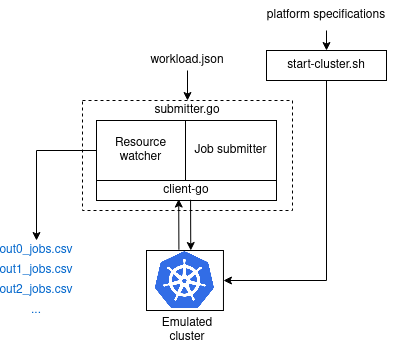
\includegraphics[scale=0.7]{./imgs/prot-k3s.png}
	\caption{An emulated experiment.}
	\label{fig:emulated-expe}
\end{figure}

Figure \ref{fig:emulated-expe} illustrates how this is done. First, we create a
k3s cluster run using docker-compose, which is a tool enabling us to
conveniently create one or several network of containers. Our cluster contains
one master node and several workers which will run our pods. Then, a Go script
which takes a Batsim workload as an input submits the jobs at the right time,
watches the cluster state regularly, and writes the ouputs to csv files --
which have the same format as Batsim's csv output files. We run each workloads
10 times in order to get statistically meaningful results, except for the
realistic workload which we only run once because it is already 10 hours long.

The emulated cluster is limited in terms of variety and capacity. First,
\texttt{start-cluster.sh} only allows the nodes to have the same amount of
available cpu, memory or storage because there was no need for any complex
system for our experiences. Secondly, the maximum amount of cpu, memory or
storage we can make available for each node is capped to the host system
capacities. For example, if the host system possesses 8 cpu cores, the nodes
will have a maximum of 8 cpu available. This will have implications when trying
to run workloads recorded on real systems: either we get to find a workload
that complies with the host system capacity (which is very unlikely), or we
adapt the workload so the jobs requirements do not exceed the host
capabilities (see section \ref{sec:studied-workloads}).

\subsection{Studied workloads} \label{sec:studied-workloads}

We consider three workloads, representing three different situations. The first
two are simplistic and very controlled, and the last one depicts a more
realistic case. In all cases the required resources are only quantified in cpu
only to simplify the study. Note that Batkube does support memory requets, we
just do not wish to add this other layer of complexity to our experiments.

\begin{itemize}
	\item A \textit{burst} workload, consisting in an important amount of
		jobs submitted at once.  200 delays with duration 170s and
		requesting 1 cpu are submitted at the origin.
	\item A \textit{spaced} workload, where jobs of the same nature are
		submitted at regular intervals.  200 delays with duration 170s,
		and requesting 1 cpu are submitted every 10s.
	\item A \textit{realistic} workload, which is a trace extracted from the  Karlsruhe Institue of Technology ForHLR II System.
\end{itemize}

The first two workloads are straight forward and could be generated with the
use of a plain text editor (understand \texttt{vim} and its macros). The third
workload required more processing to be obtained.  

\subsubsection{Standard Workload Format processing}

Batsim provides a tool to translate SWF files to its own json definition. It
also works as a workload preprocessor, although we want to process SWF files
very specifically to suit our needs which is why a custom script was
implemented.

First, a trace in standard workload format (swf) was obtained on a web
archive\footnote{https://www.cs.huji.ac.il/labs/parallel/workload/logs.html}.
The chosen workload was \texttt{KIT-FH2-2016-1.swf} (we give the file name for
the reader to find the workload on the archives) because it is the most recent
and is relatively lightweight. It is composed of 114,355 jobs spanning over 19
months. Secondly, \texttt{evalys}\footnote{https://github.com/oar-team/evalys}
allowed us to extract a subset of this workload lasting for a given period of
time and with a given mean utilization of the resources. We chose a period of
10h with 80\% utilization of the resources so as to keep reasonable experiment
durations -- Later on we experiment with larger workloads to test out Batkube's
limits in terms of scalability.  The third step is translating this extracted
workload to a \texttt{json} file that can be read by Batsim, which is done with
a script written in Go.

After extracting this subset, we are left off with a workload containing jobs
spanning up to 45h and using up to 24048 cpu (or cpu cores), which is undoable
at our scale on our emulated cluster. We need to trim job durations as well as
cpu usage, as we are limited in cpu by the host machine. This is done during
the translation to the \texttt{json} format. The durations are trimmed down to
a maximum of one hour and the cpu usages are normalized so the maximum amount
of cpu requested equals the amount of cpu available per node on the host
machine. Otherwise, the job would not be schedulable which would not present
much interest. We end up with a trace composed of 39 jobs spanning over 10
hours, with a maximum job length of one hour and cpu usage ranging from 0
(excluded) to 5.9 (even though the host machine had 6 cores, Kubernetes
scheduler did not allow for a job to be scheduled on a node it would use 100\%
resources of).

\subsection{Studied platforms}

The platform used for the first two workloads, \textit{burst} and
\textit{spaced} is composed of 16 nodes each heaving one cpu. For the
\textit{realistic} workload however, we use a single node composed of six cores
for the following reasons.

First, the host machines where the experiments were conducted had six cpu cores
available. This means that if we want to be able to run an emulated cluster
equivalent to this platform we can't exceed six cpu per node.  We use the
maximum amount of available cores in order so as not to obtain too low values
when normalizing the resource requests on the jobs. Indeed, Kubernetes only
allows for a precision of 1 milicpu, so any value bellow that is not considered
a significant number. Normalizing on six cpus instead of one allows us to get
more significant number. Also, only one node gives us a satisfactory overall
resource usage: with more than one node one resource is almost always available
making the scheduling operations trivial.

\section{Study of the simulator parameters}

The simulator has a few parameters that impact the simulation speed and
accuracy. The objective is to study the effects of these parameters on the
simulation to better understand the scheduler behavior when running in
coordination with Batkube.\\

The objective here is to fine tune the parameters in order to find a compromise
between accuracy and scalability. We want to know which combination lead us to
the most stable results, while keeping simulation time as low as possible.

The parameters are:
\begin{itemize}
	\item The \textit{minimum delay} we have to spend waiting for the
		scheduler.
	\item The \textit{timeout} value when waiting for scheduler decisions.
	\item The \textit{maximum simulation time step}, which is the maximum
		amount of time Batsim is allowed to jump forward in time.
\end{itemize}

We first study these parameters one by one by fixing the other parameters to
some other value, then we study what effects these parameters have in respect
to one another, and finally we conduct scalability experiments to test
Batkube's stability and performances on large workloads.

\subsection{Minimum delay}

Earlier in the development of batkube we noticed that not leaving enough time
to the scheduler each cycle lead it to crashes and deadlocks, ultimately
failing the simulation. This time is independent from any decision making we
would receive from it which is why it is called \textit{minimum wait delay}
instead of a plain \textit{timeout} - which is in fact another parameter we
will study later.

For each workload, we compute the crash rate every 5ms, from 0ms to 50ms. Each
point is made by running the simulation 15 times and recording the exit code as
well as the simulation time. The other parameters are: \texttt{timeout=20ms};
\texttt{max-simulation-timestep=20s}. As we will see later those do not offer
acceptable simulation results but they allow us to run prompt simulations, as
accuracy do not concern us here.\\

\begin{figure}
	\centering
	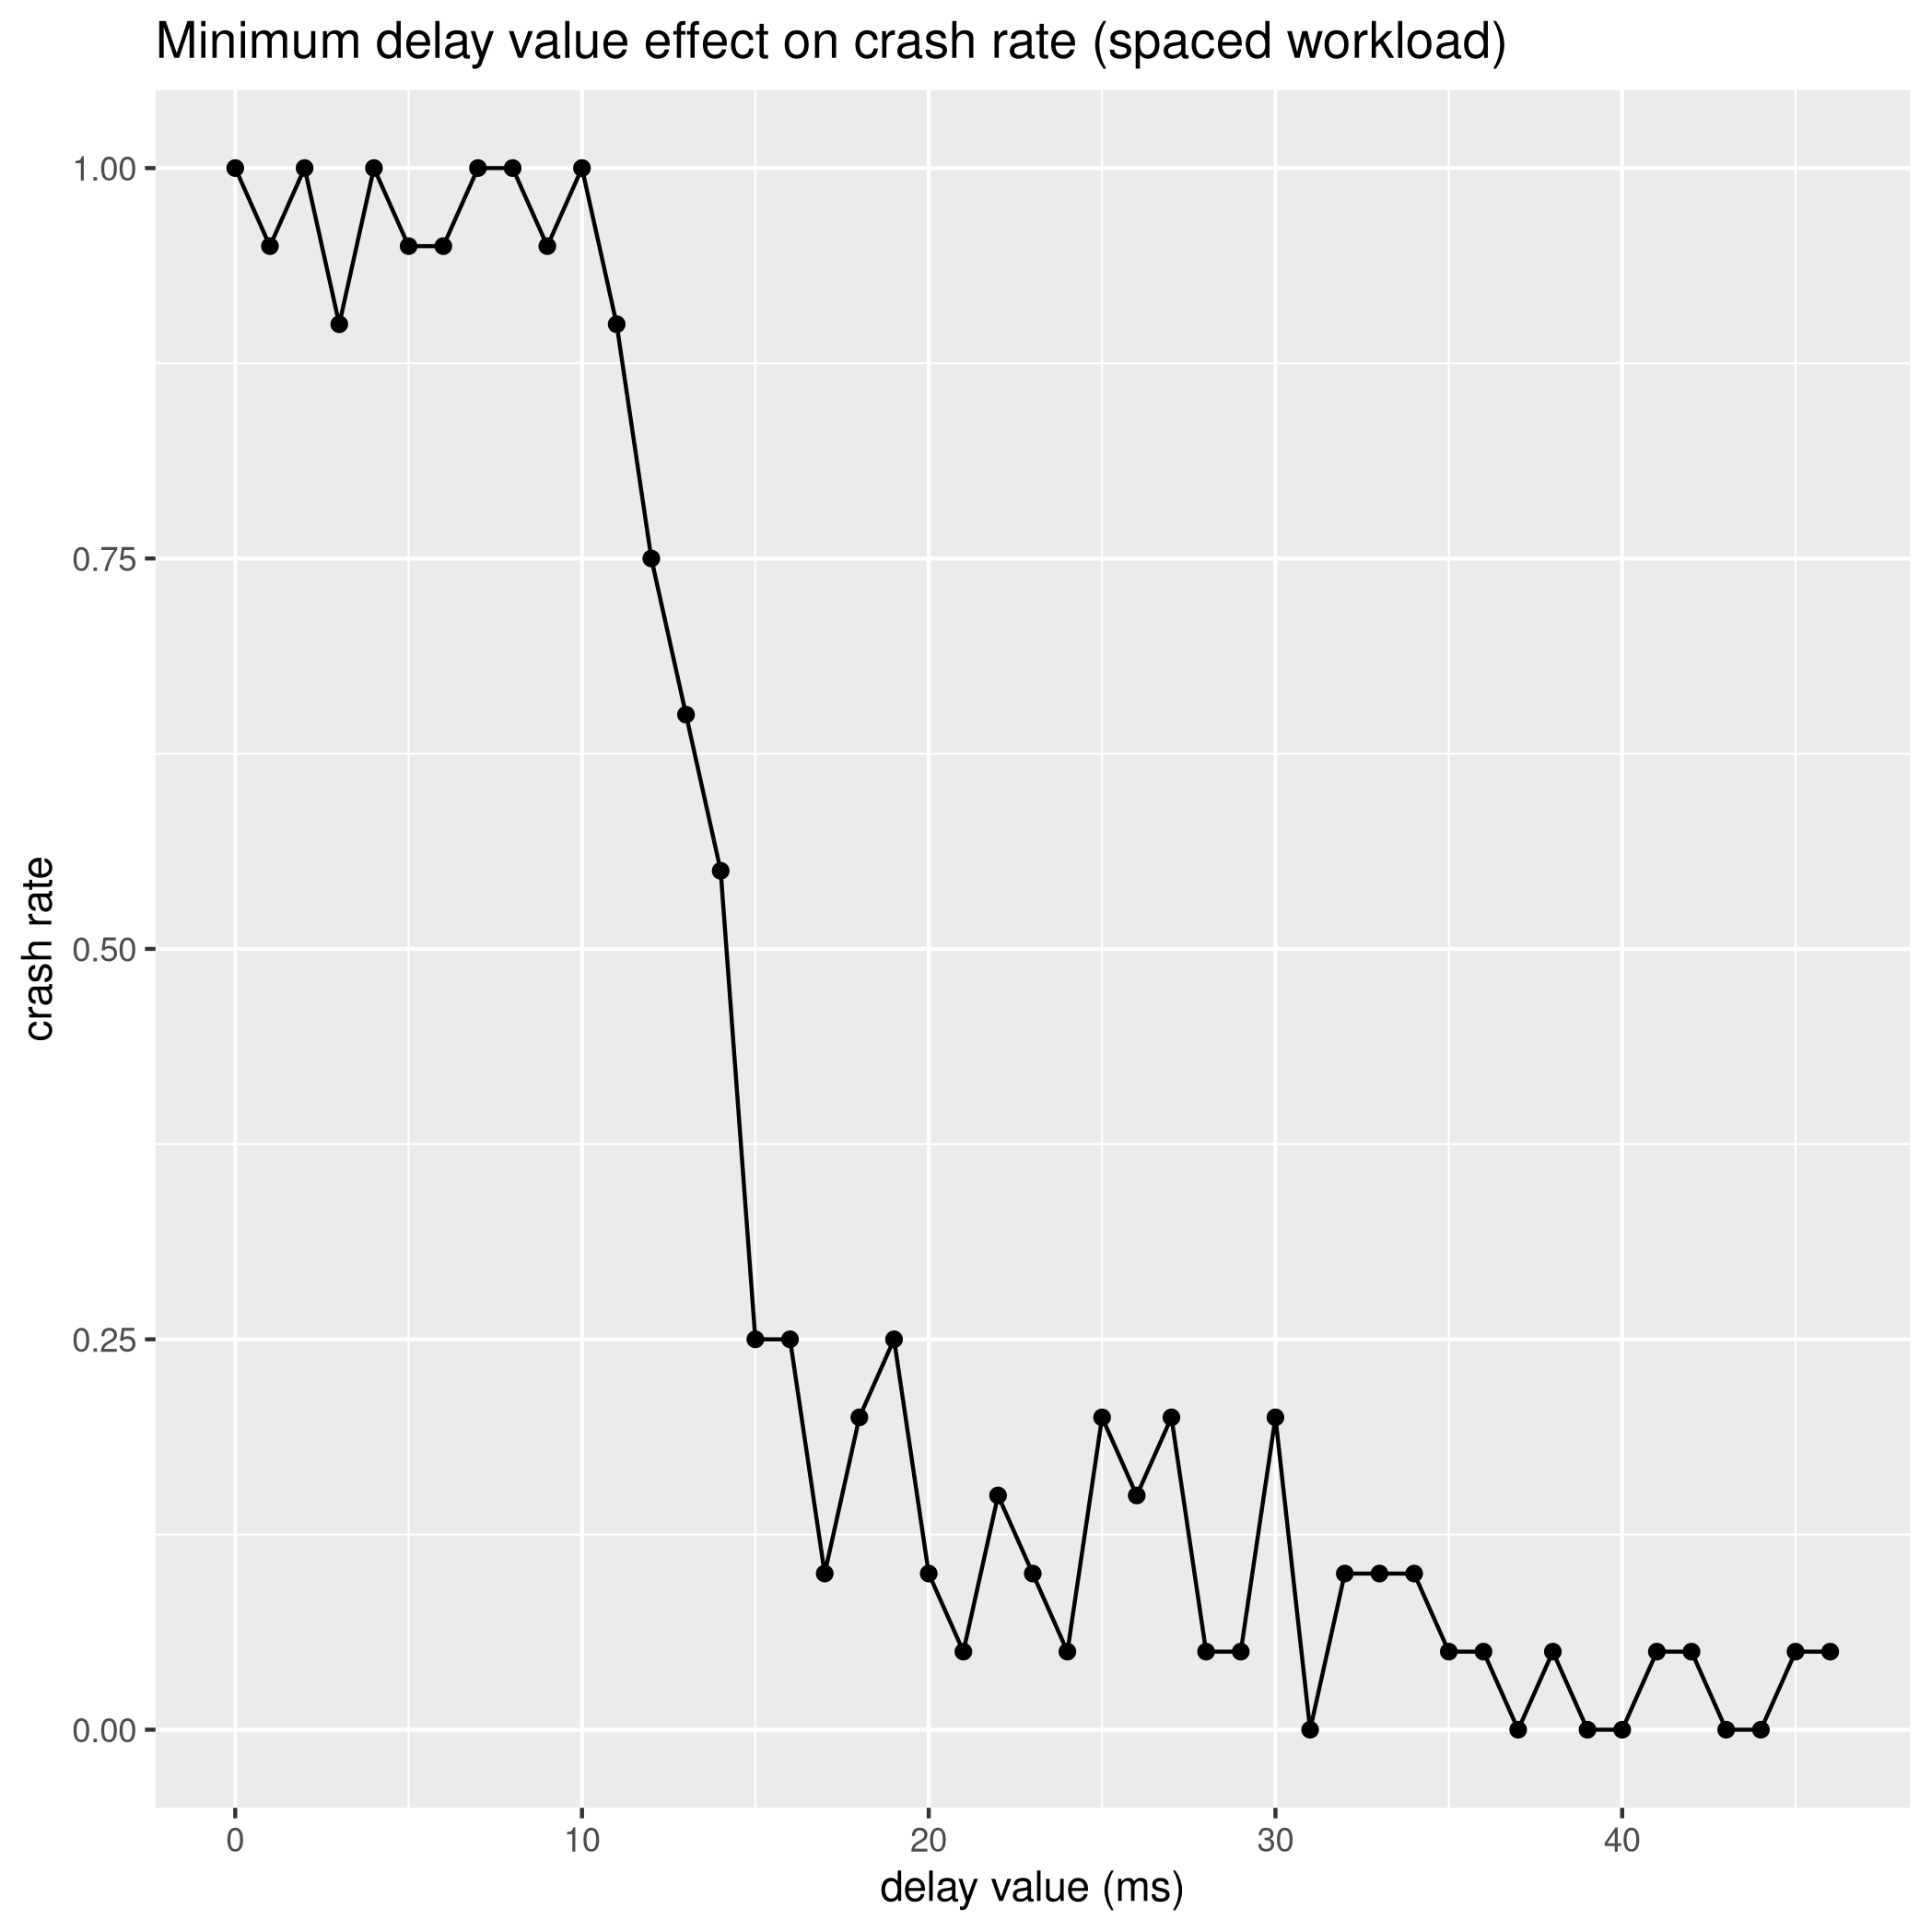
\includegraphics[width=0.45\textwidth]{imgs/min-delay_spaced_200_delay170_crash_old.png}
	\caption{Crash rate of the simulations against minimum delay.}
	\label{fig:min-delay_crash}
\end{figure}

\begin{figure}
	\centering
	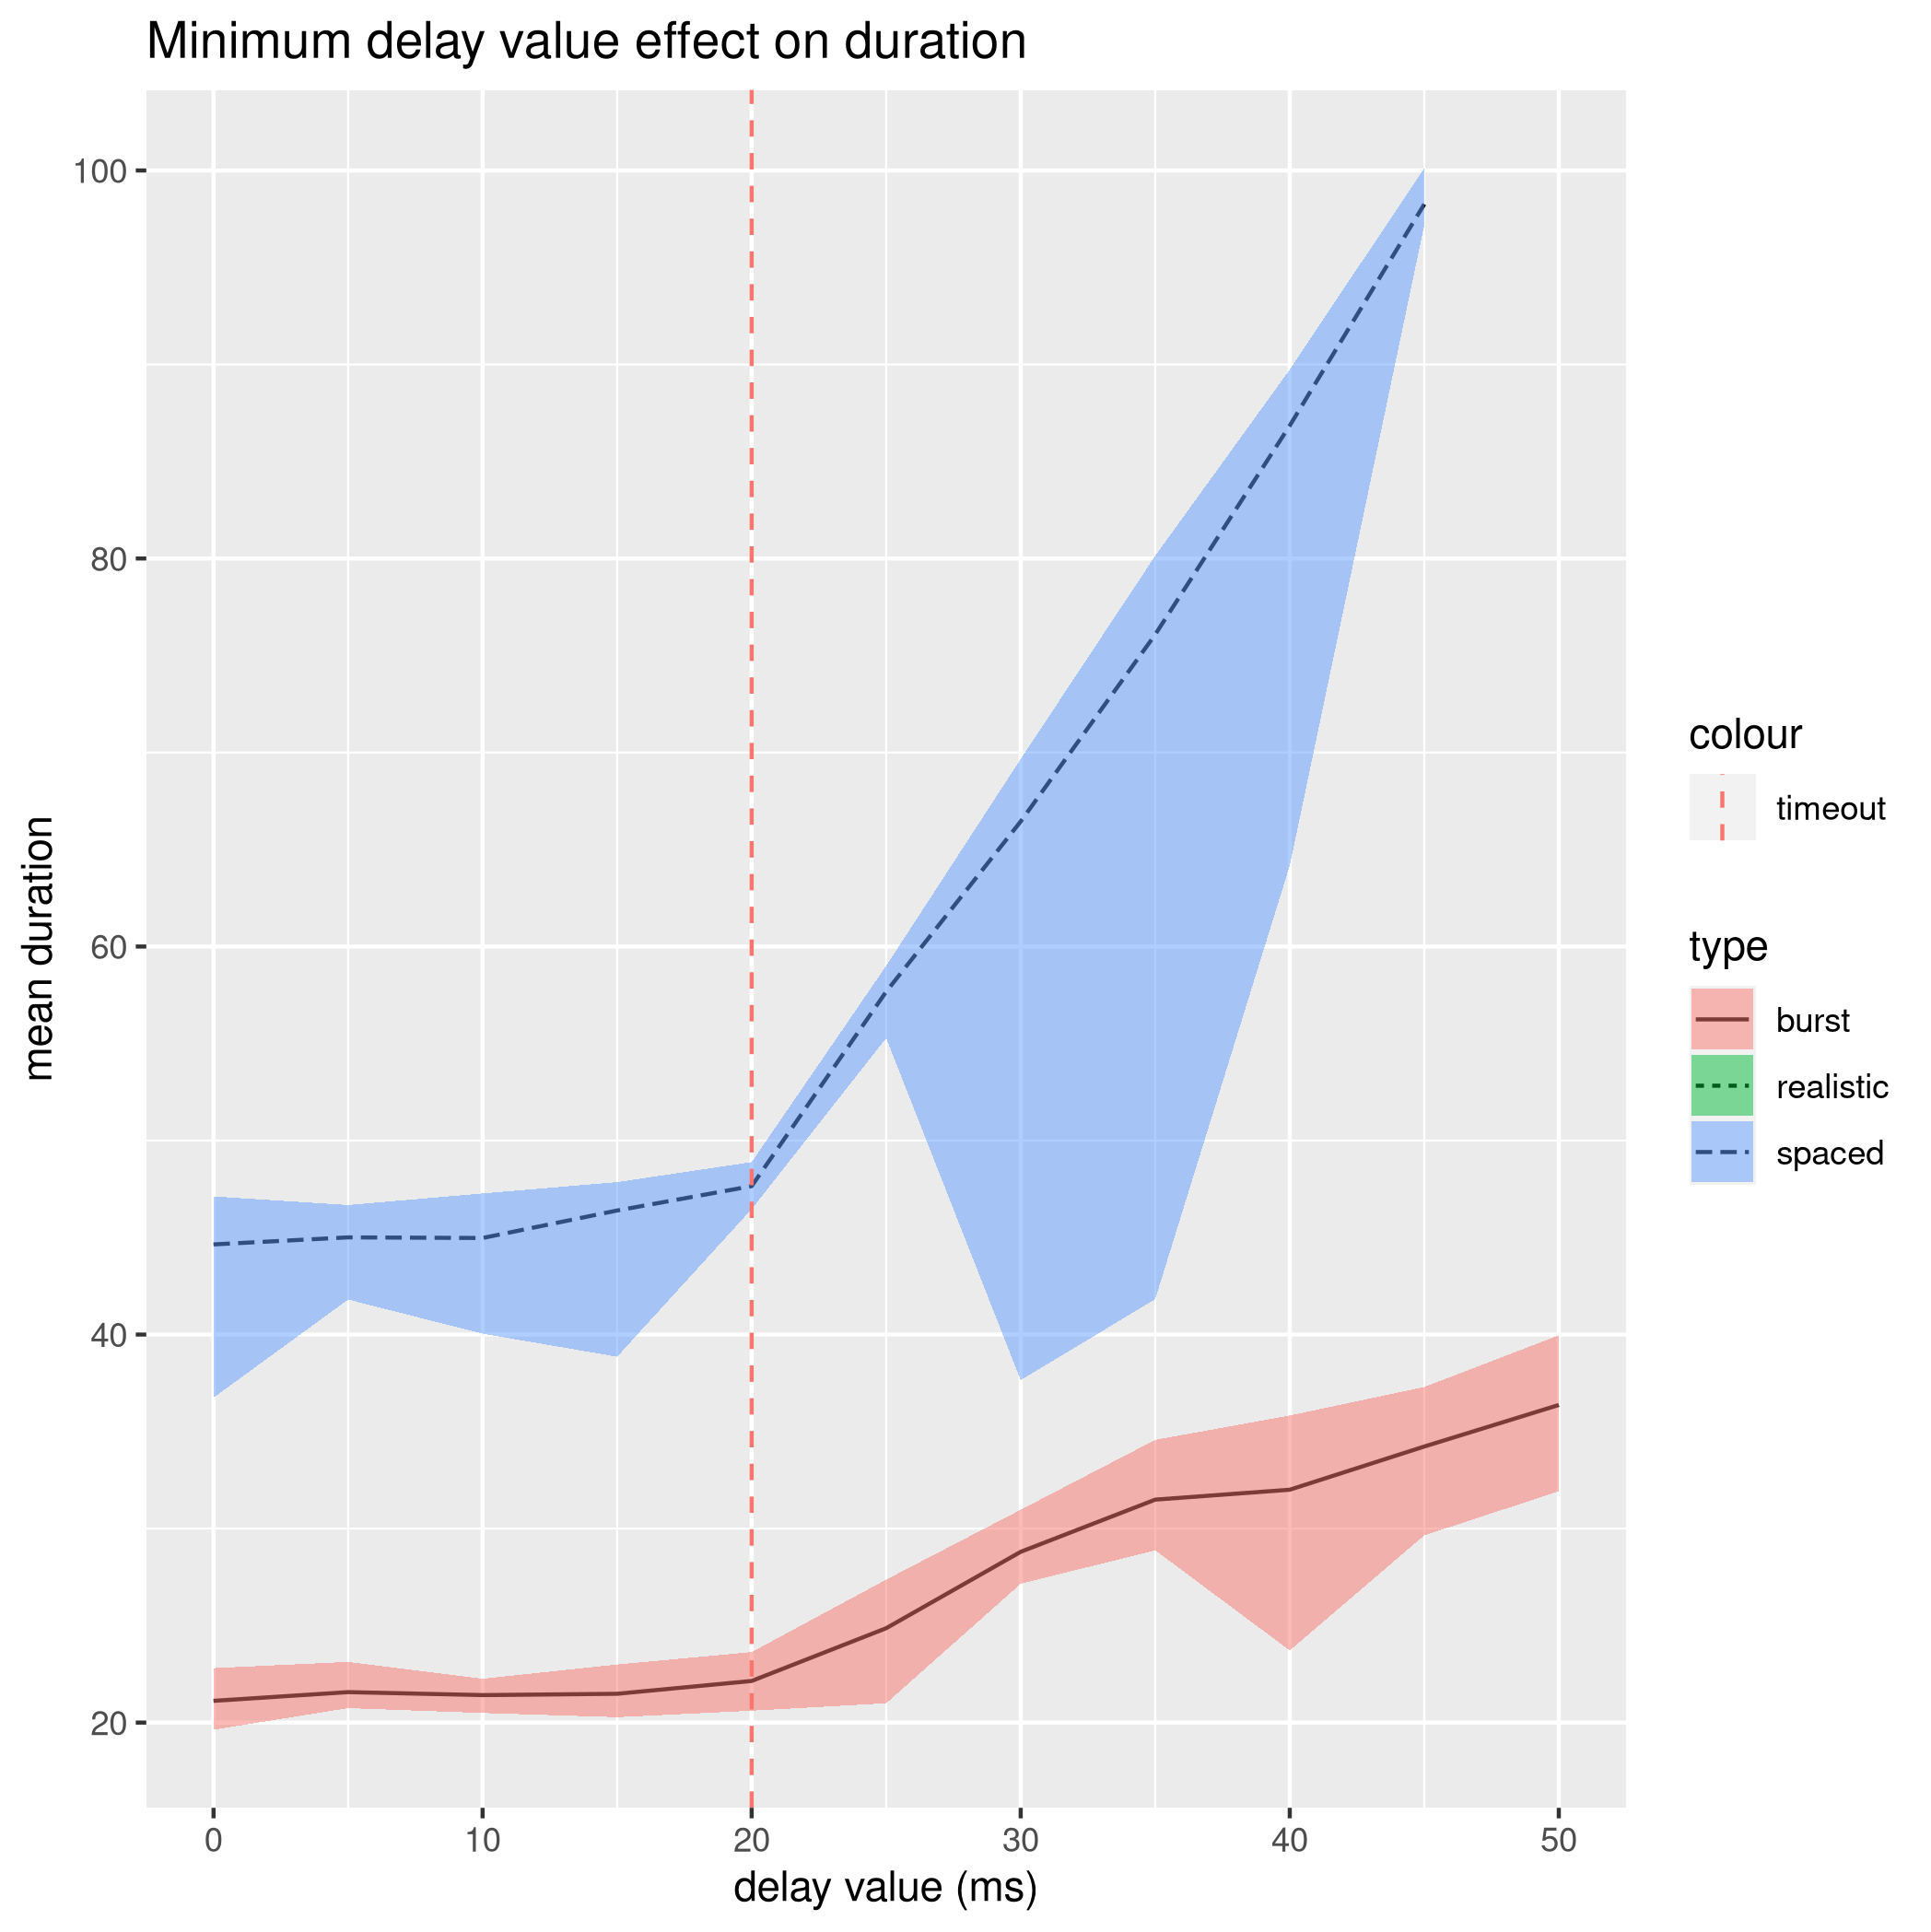
\includegraphics[width=\textwidth]{imgs/min-delay_duration.png}
	\caption{Mean duration of the simulations (in case of success) against minimum delay. Error bars show confidence intervals at 95\%.}
	\label{fig:min-delay_duration}
\end{figure}

As we can see on figure \ref{fig:min-delay_crash}, the crash rate decreases
dramatically as soon as the minimum delay reaches a certain threshold, which
here is 10ms.  This crashing issue though was resolved with an update of the
scheduler : the success rate flattens out at 100\% -- or around 100\%. Then,
with earlier versions of the scheduler, the user may have to adjust the minimum
delay in order to run simulation smoothly. 

We also observe on figure \ref{fig:min-delay_duration} -- which was made with
an updated scheduler -- a prompt increase in simulation time from delay value
20ms. This is due to the fact that the \textit{timeout} value is 20ms, which is
reached most of the time because the vast majority of the calls to the
scheduler do not result in a decision making. After this value, we notice a
direct correlation between \textit{minimum delay} increase and simulation time
increase. It follows that the best choice for the \textit{minimum delay} now is
zero, and we will use this value for the rest of the experiments.


\subsection{Timeout}

This value is the maximum amount of time we leave for the scheduler to react. A
\texttt{timeout value} not large enough may lead to inaccuracies in the
simulation: for example, if the scheduler needs 30ms to make a decision upon
reception of a message, and the value of the timeout is 20ms, Batkube will
receive the decision on the next cycle which may happen several dozens of
seconds later (depending on the \textit{maximum simulation time step} value).
On the other hand, a \textit{timeout value} too large will induce longer
simulation times. Indeed, once the simulator was given enough
time to process a message, any time following is spent idling. We want to
measure which \texttt{timeout value} is just enough for the scheduler to be
able to make a response without spending any time idling.

We run each workload with a \texttt{timeout value} ranging from 0ms to 100ms,
with a step of 1ms. Each time we measure the duration of the simulation as well
as the makespan and the mean waiting time. The latter two will enable us to
compare the results against the emulated results in order to estimate the
accuracy of the simulation. The other parameters are set to:
\texttt{min-delay=0ms}, \texttt{max-simulation-timestep=20s}

\begin{figure}
	\begin{subfigure}{.5\textwidth}
		\centering
		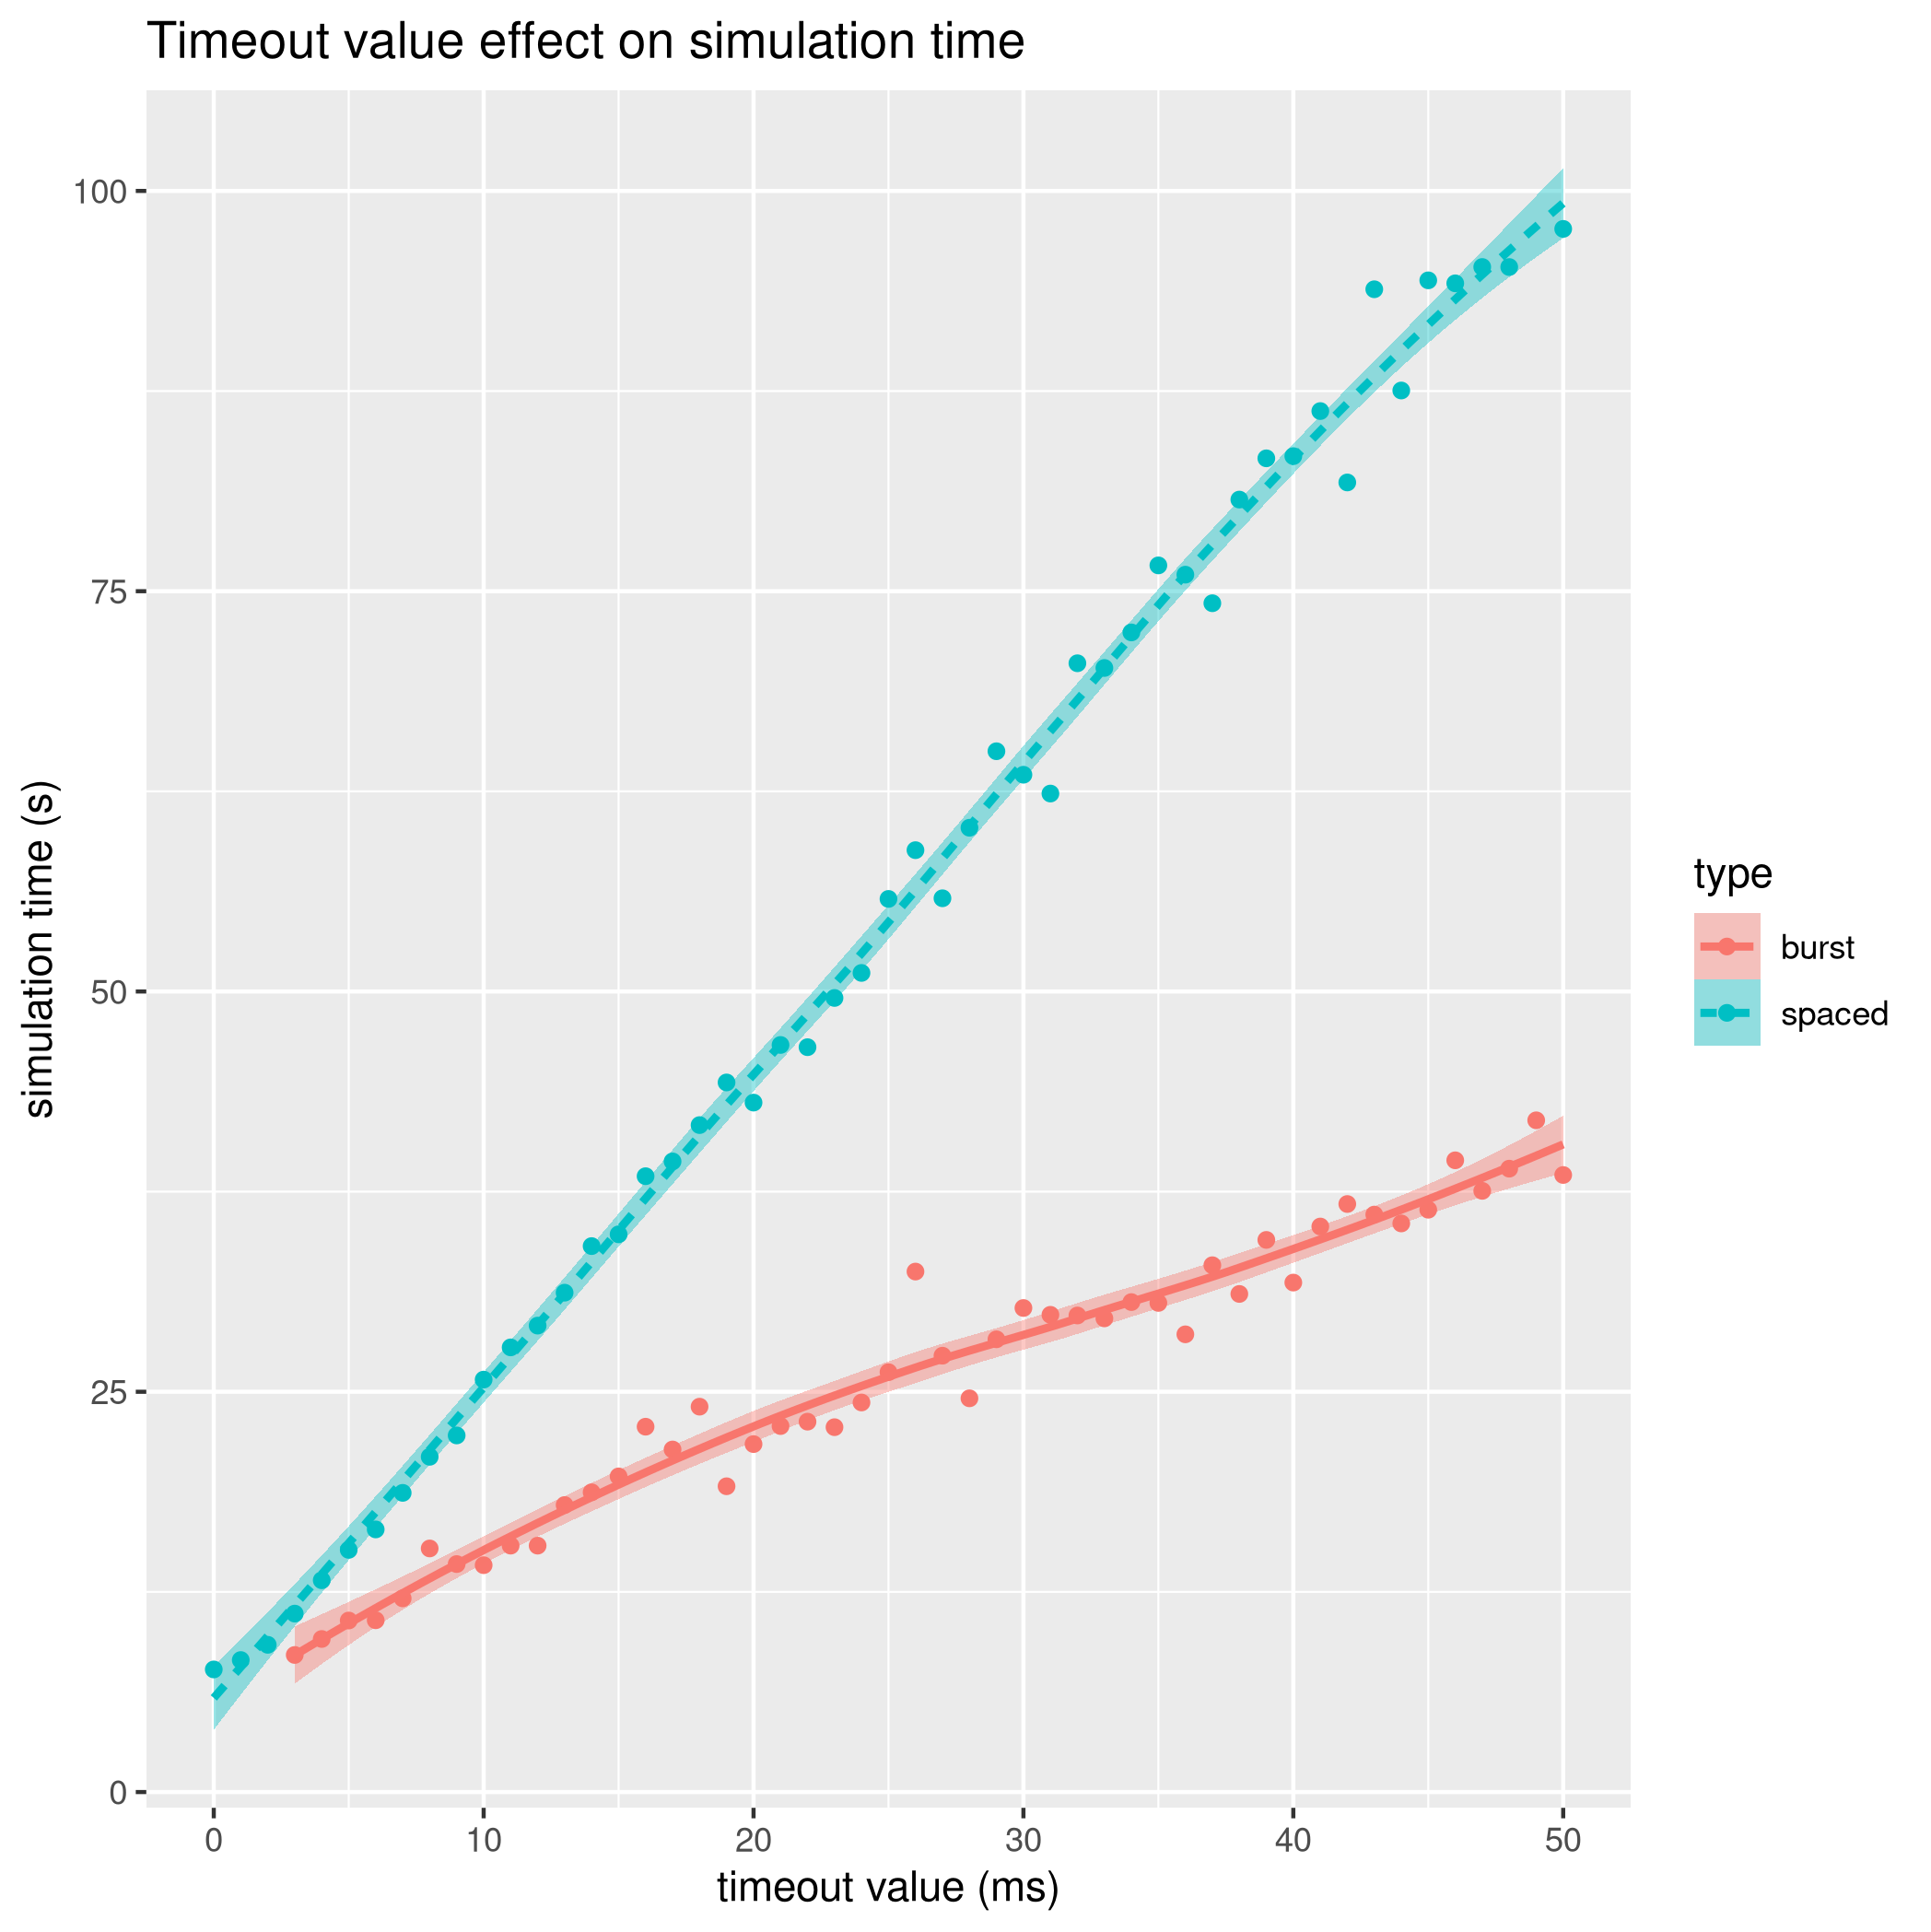
\includegraphics[width=\linewidth]{imgs/timeout_duration.png}
		\caption{}
		\label{fig:timeout_duration}
	\end{subfigure}
	\begin{subfigure}{.5\textwidth}
		\centering
		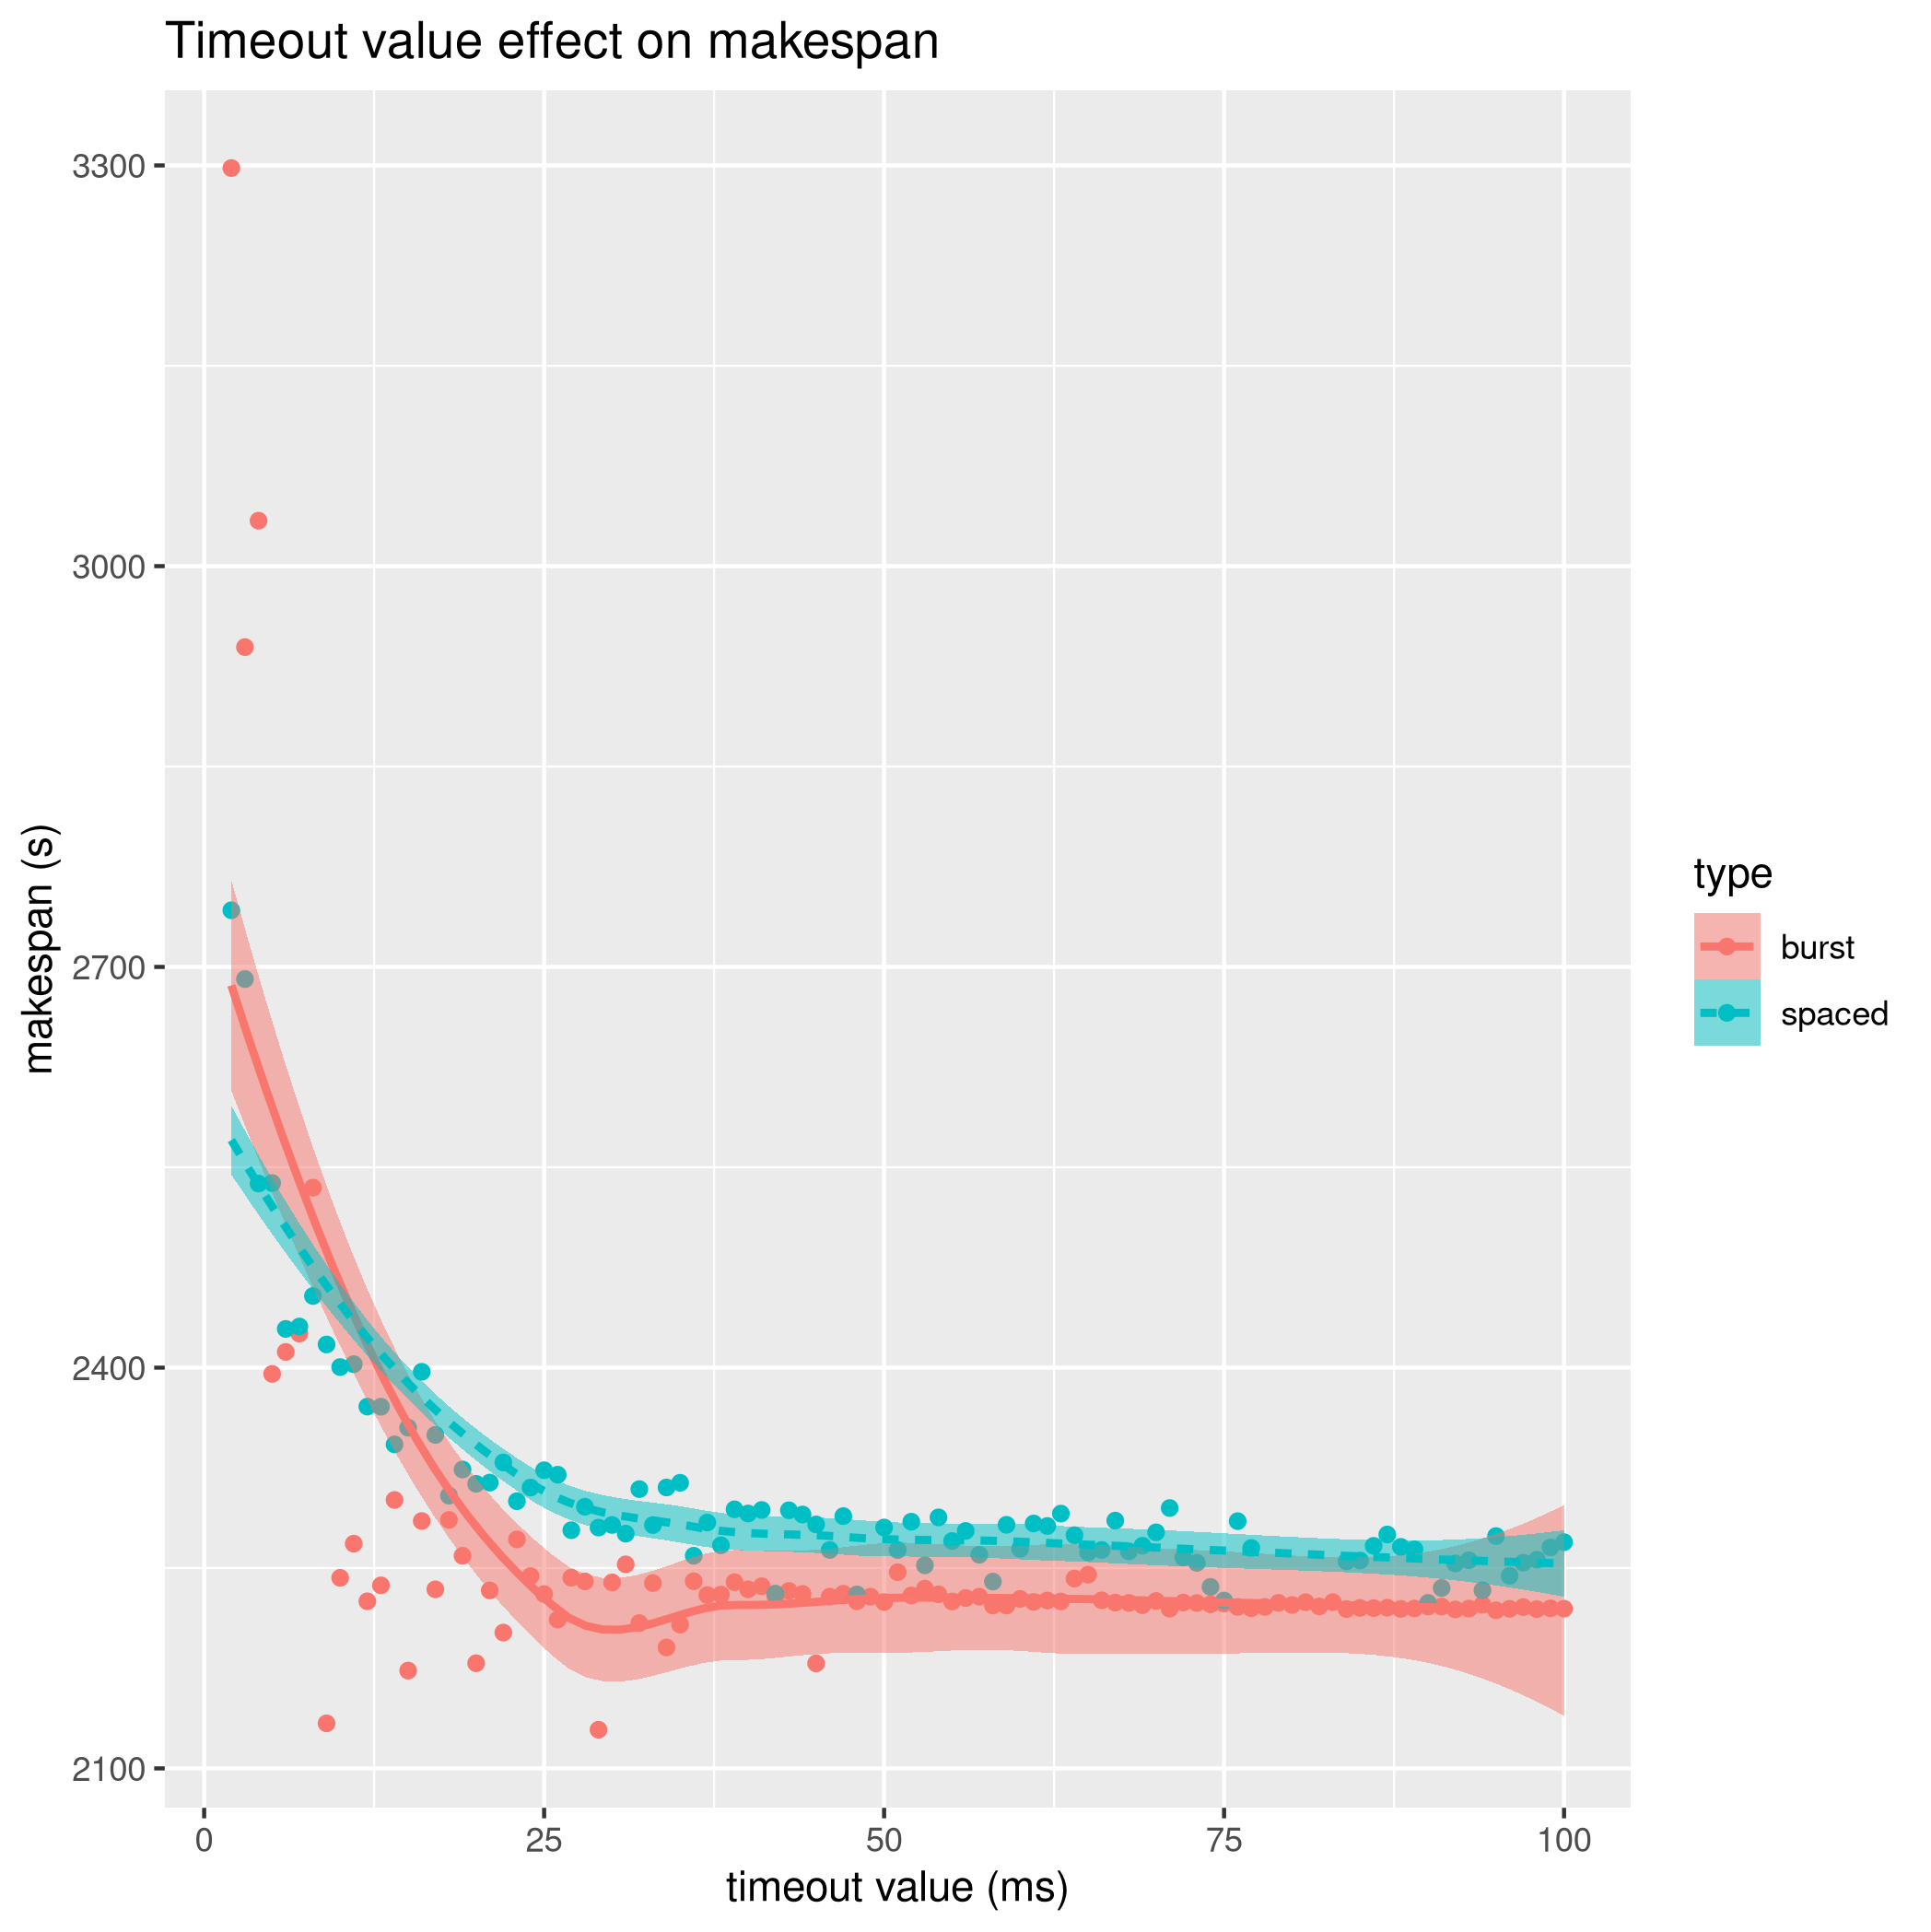
\includegraphics[width=\linewidth]{imgs/timeout_makespan.png}
		\caption{}
		\label{fig:timeout_makespan}
	\end{subfigure}

	\centering
	\begin{subfigure}{.5\textwidth}
		\centering
		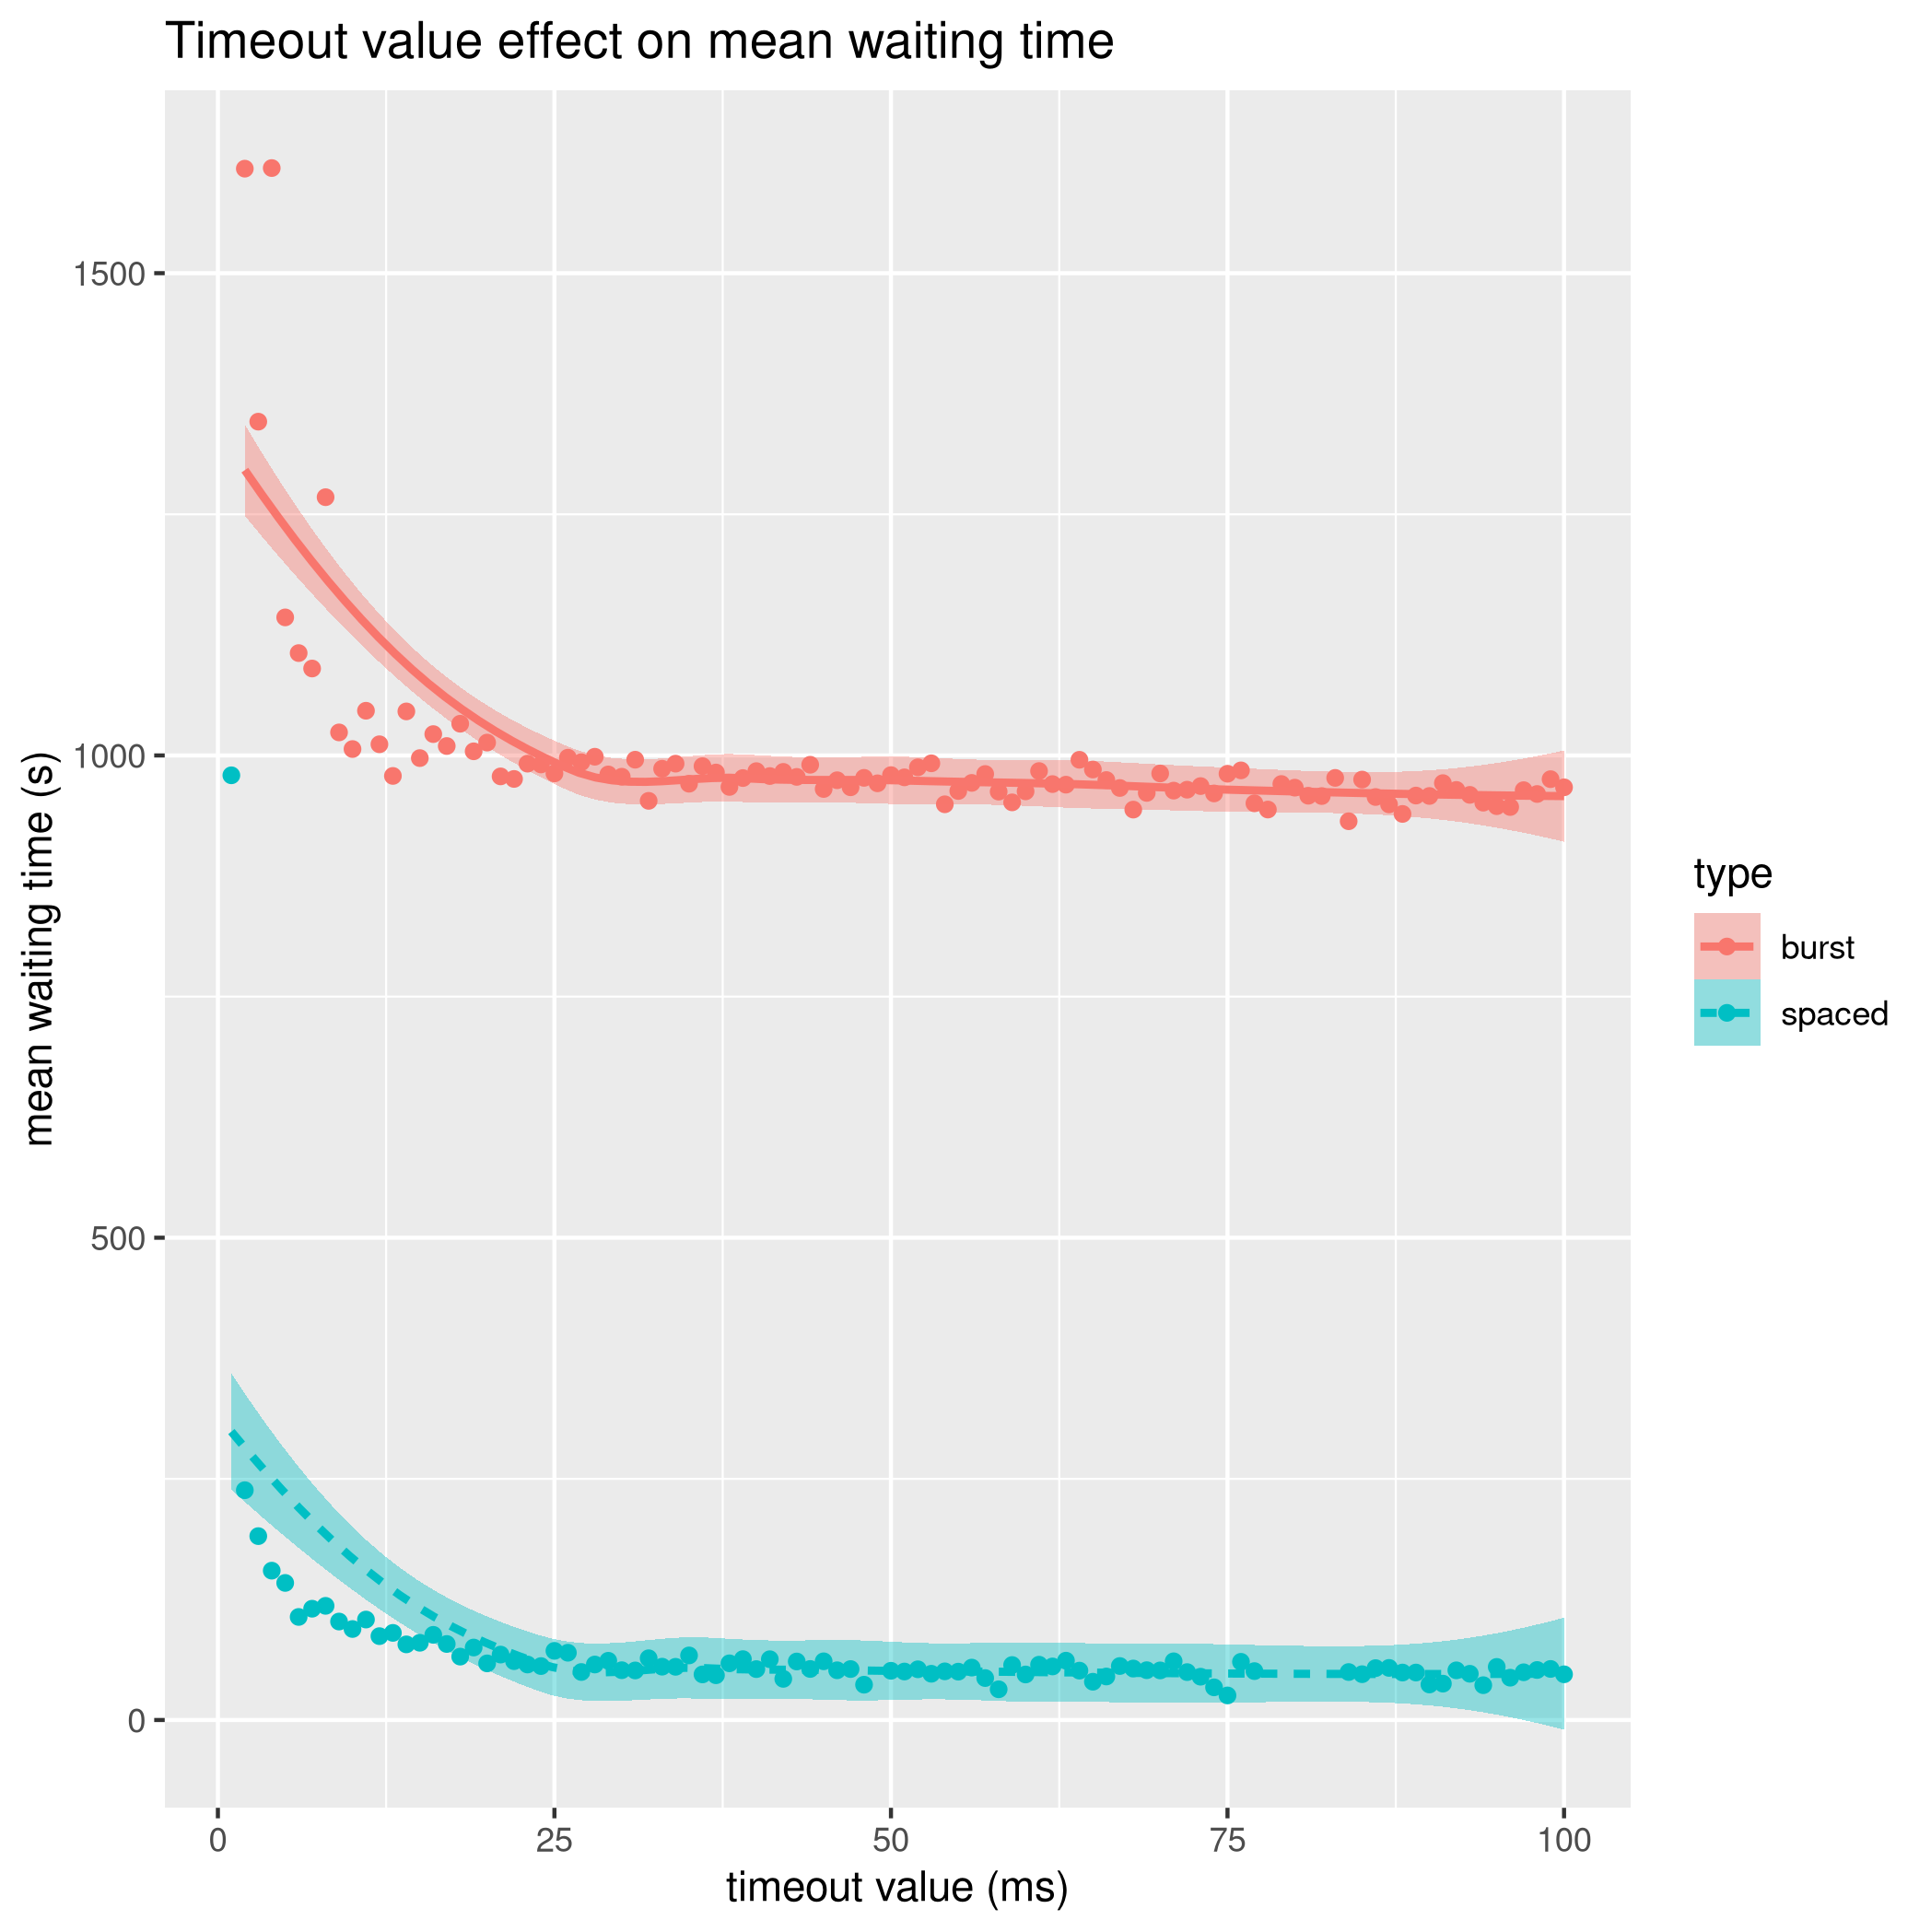
\includegraphics[width=\linewidth]{imgs/timeout_mwt.png}
		\caption{}
		\label{fig:timeout_mwt}
	\end{subfigure}
	\caption{Effect of the timeout value on the simulation}
	\label{fig:timeout}
\end{figure}

TODO: redo the simulations for the realistic wl, removing some values of
timeout and adding repetition to show aggregated metrics. (non aggregated ones
are too dispersed)

TODO: \ref{fig:timeout_duration} does not have the same scale on the x axis as the others.

TODO: Gantt charts to show the gaps.

As we expected, a \textit{timeout value} too low results in the scheduler
missing a few cycles each time it wants to communicate a decision making, thus
increasing the makespan and mean waiting time.  As the \textit{timeout}
increases, it reaches a point where the scheduler consistently sends decisions
in the same cycle as the one where it has received the message that triggered
the decision making. After this point though the curves keep decreasing,
showing that the gaps keep receding afterwards. However, the gain in accuracy
is shallow and considering that there is, again, a direct correlation between
the \textit{timeout value} and the simulation time, it is desirable to keep
this value at the limit where the results start to stabilize.  In this case,
according to figure \ref{fig:timeout_makespan}, \texttt{timeout-value=50ms}
seems like a decent compromise between accuracy and scalability.

With such simple workloads and platforms, the decision making time is very low
(it is but a matter of milliseconds), but we can imagine it may reach much
higher values given a bigger platform and more complicated workload.

\subsection{Maximum simulation time step}

Having a high maximum time step value will allow Batsim to jump forward further
in time. This may result in skipping scheduler decisions that could have been
made in the mean time, delaying them to when Batsim decides to wake up. We
expect increasing this value to have an analogous effect to the timeout value:
higher simulation speed, but also decreased accuracy due to gaps (delays) in
the decision process.

To experiment with the maximum time step effect on the results we obtain, we
run each workload with different values of \texttt{max-simulation-timestep}
following a logarithmic scale. The other parameters are fixed to
\texttt{min-delay=0s}, \texttt{timeout=50ms}. Also, the
\texttt{base-simulation-timestep} was lowered to 10ms in order to test lower
values of the maximum timestep (compared to the previous 100ms).

\begin{figure}[]
	\centering
	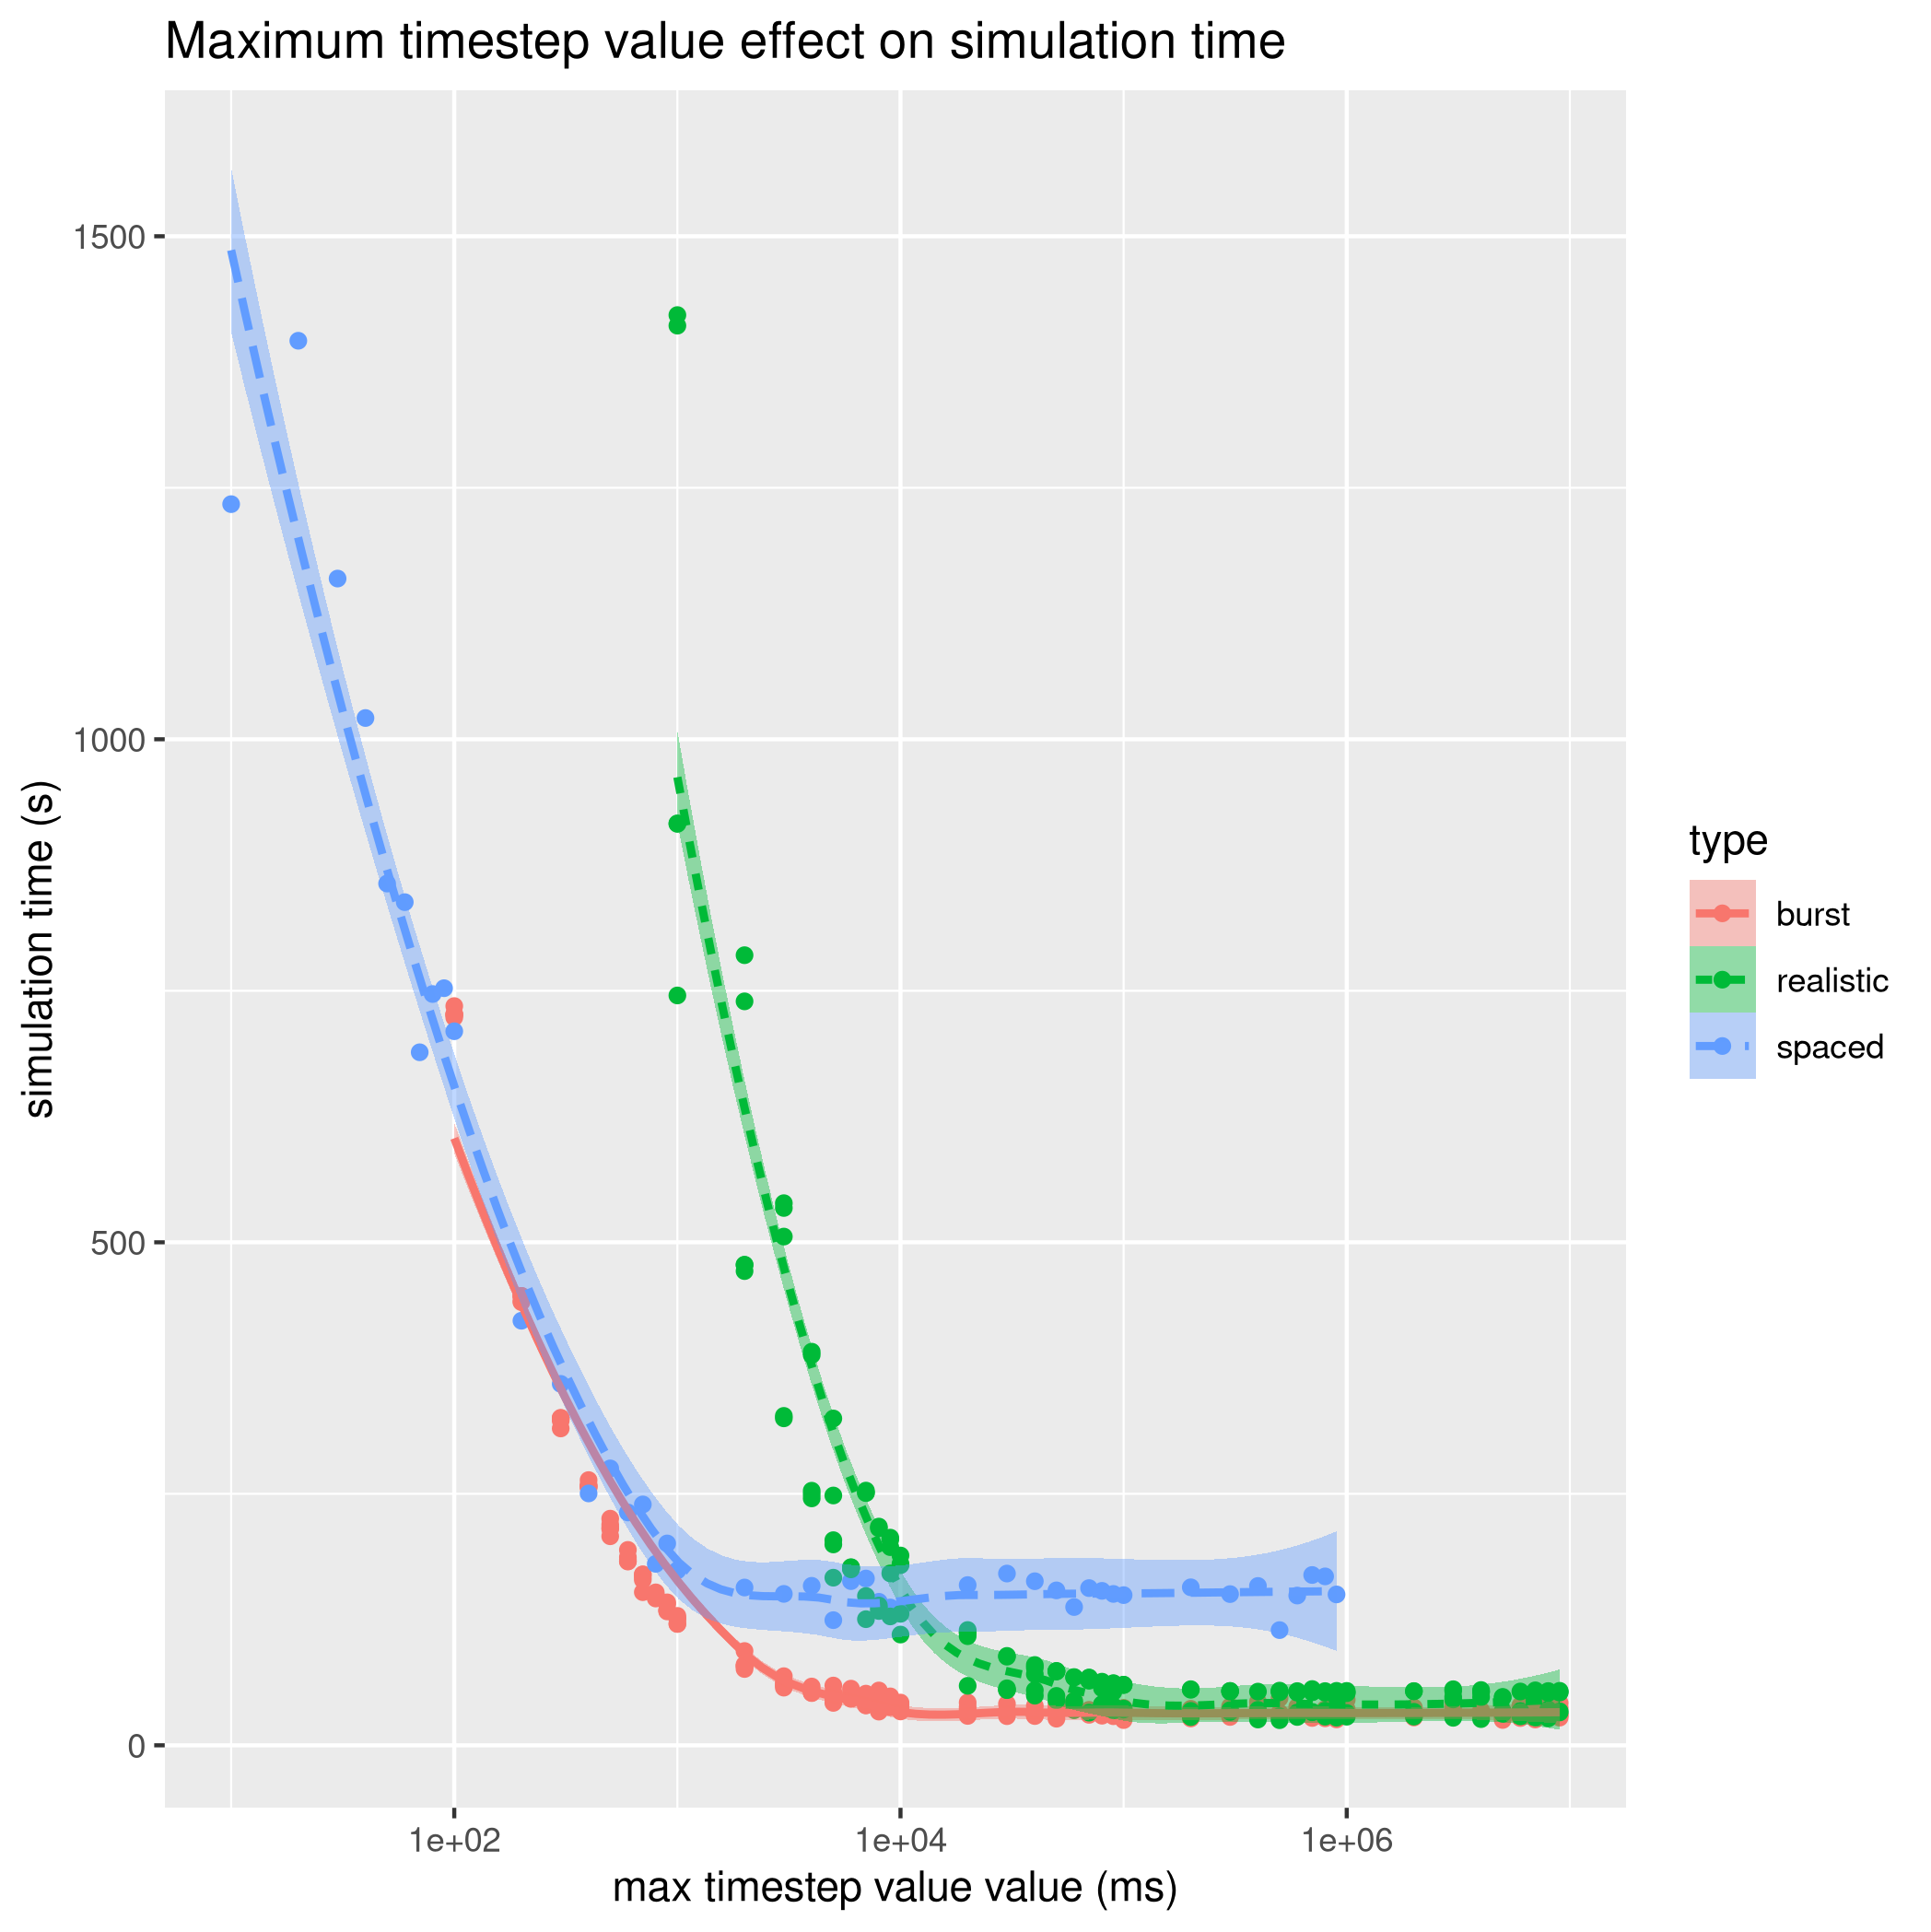
\includegraphics[scale=0.5]{imgs/max-timestep_duration.png}
	\caption{Effect of maximum timestep on simulation time}
	\label{fig:max_timestep_duration}
\end{figure}

\begin{figure}[]
	\centering
	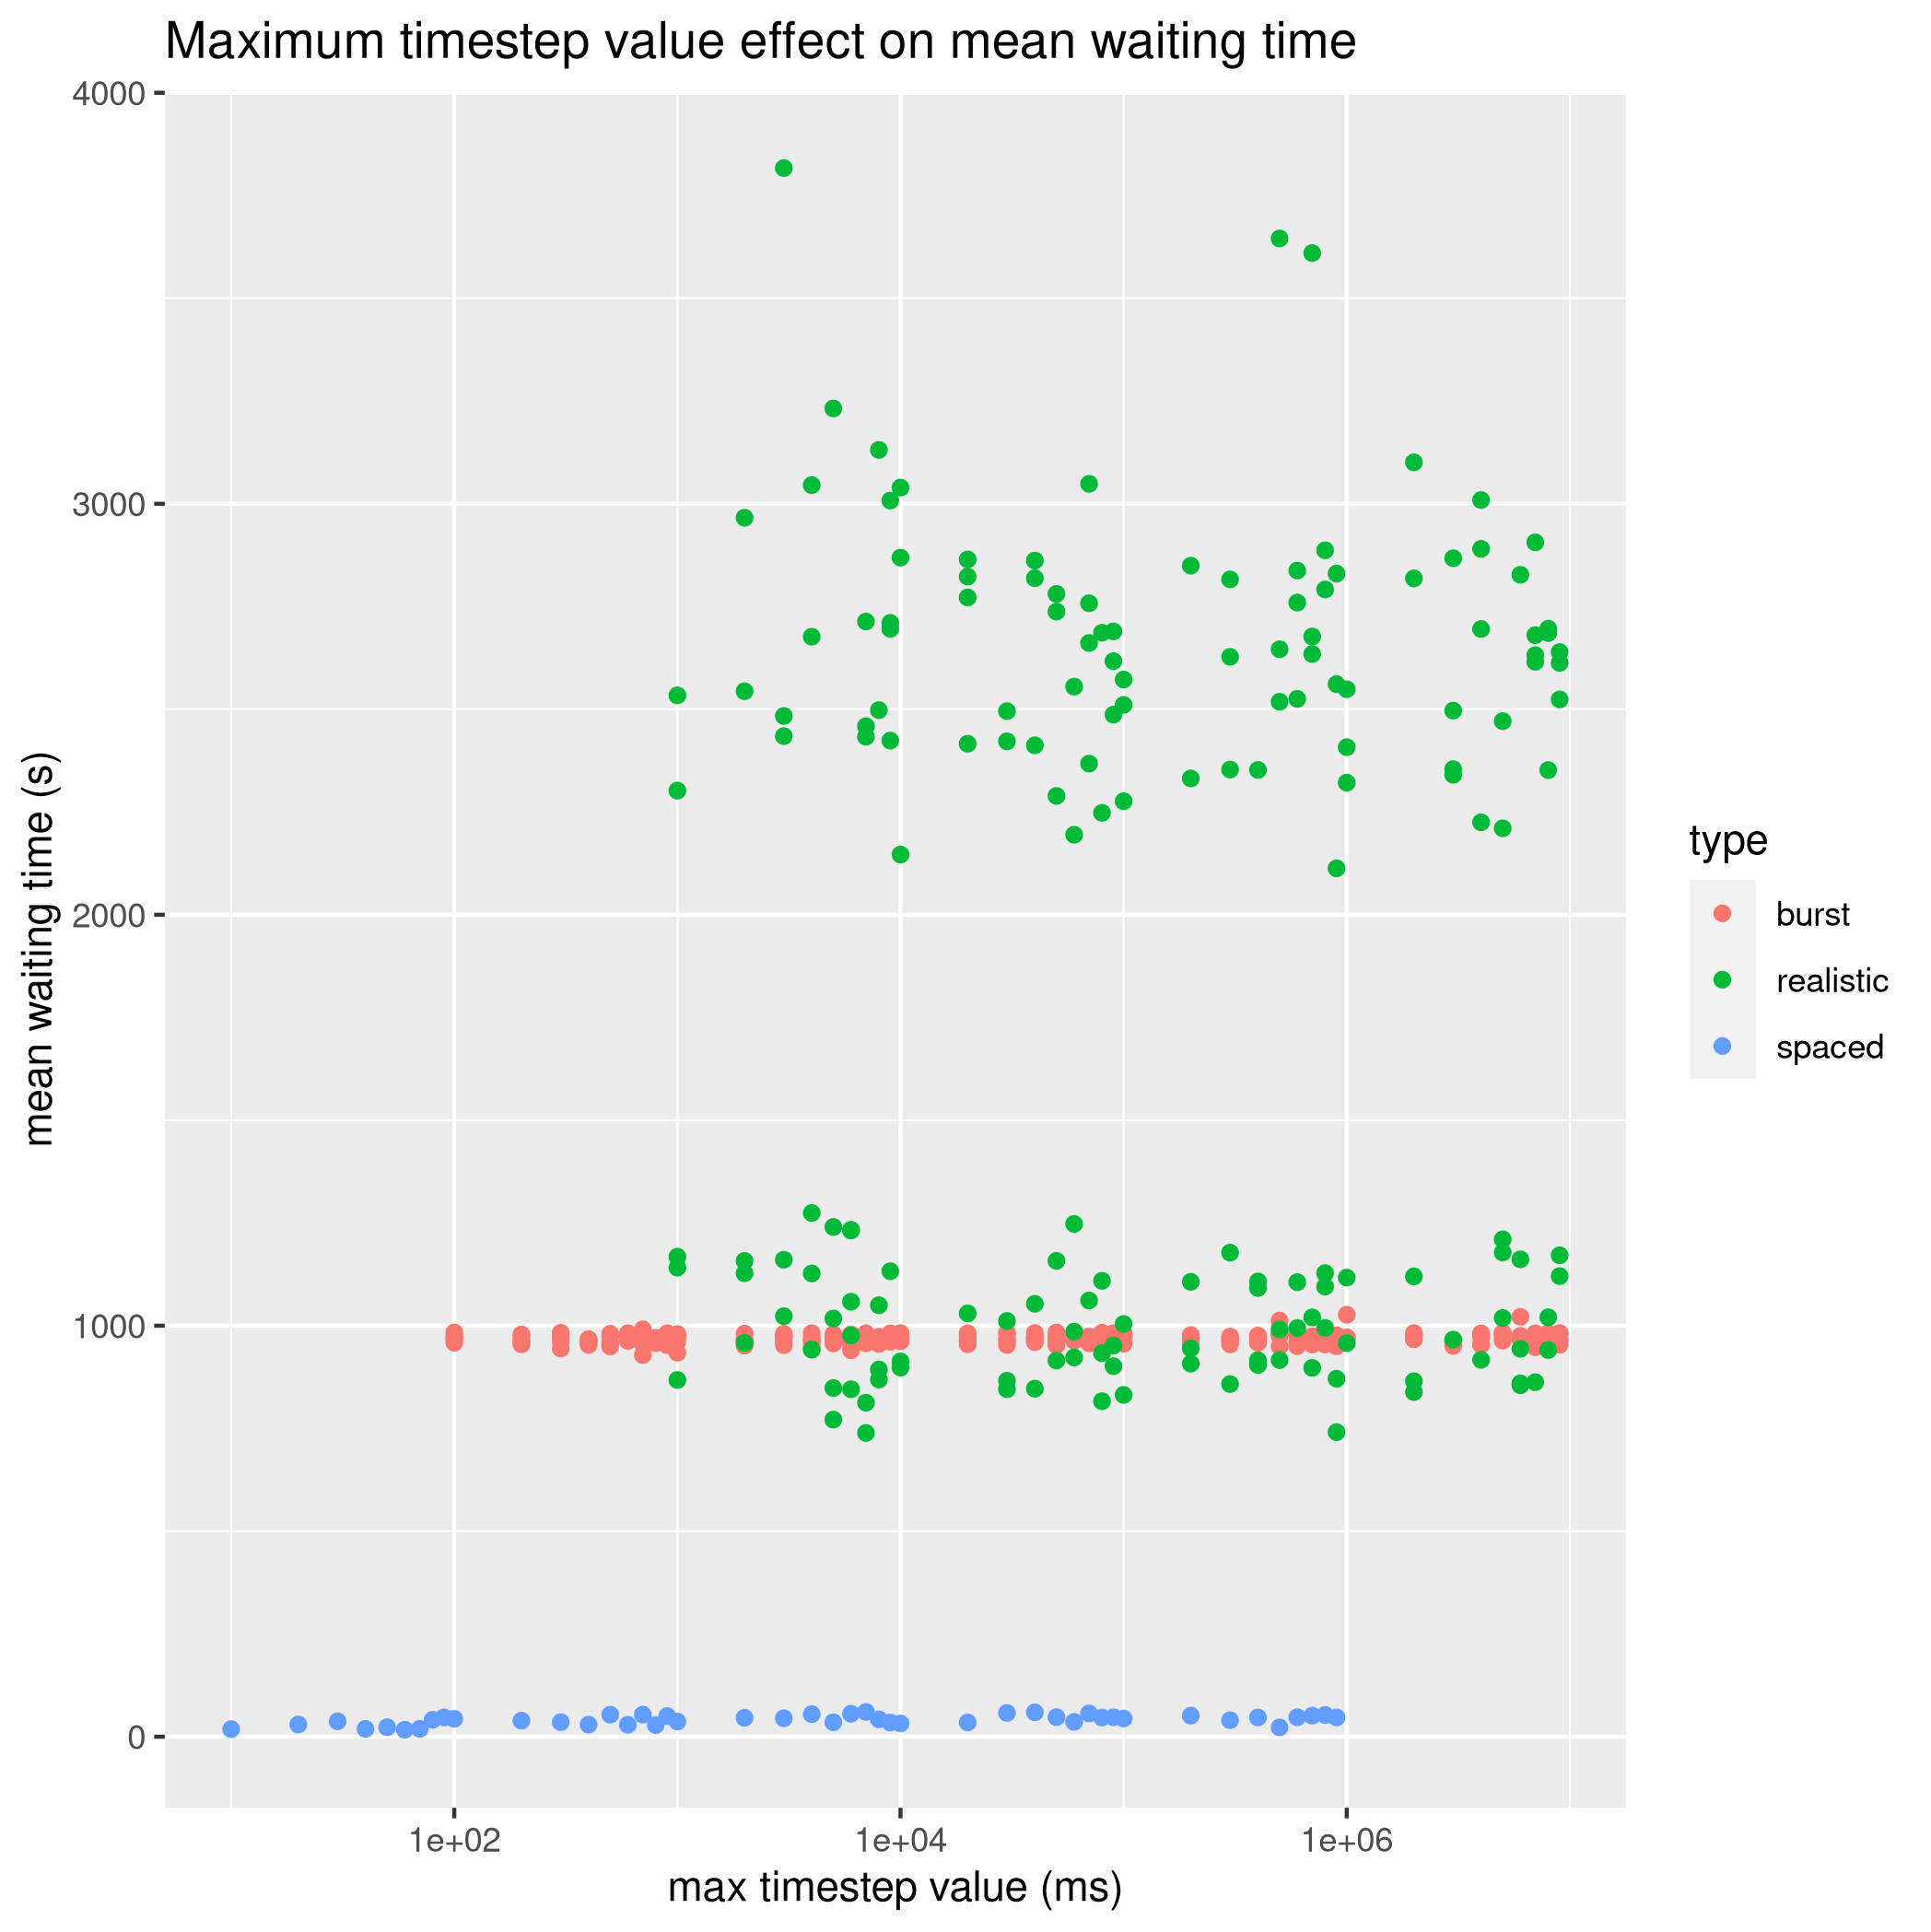
\includegraphics[scale=0.5]{imgs/max-timestep_mwt.png}
	\caption{Effect of maximum timestep on mean waiting time}
	\label{fig:max_timestep_mwt}
\end{figure}

As expected, the simulation time decreases drastically when the maximum
timestep increases. Still, this value reaches a minimum eventhough the maximum
timestep keeps increasing. This happens because Batsim events are only so far
appart in the simulation, and Batsim will always wake up before the maximum
timestep is reached.

TODO: redo the experiment for the spaced wl and redo the graph for makespan (do
not put all three wl on the same graph because the scale is so different).

\subsection{Parameters inter dependency}

Studying the parameters independently is not enough, we need to study their
impact relatively to each others.

For instance, the \textit{maximum simulation time step} and the
\textit{timeout} value are tightly linked together regarding their effect on
accuracy. Both decreasing \textit{timeout} and increasing \textit{maximum
simulation time step} will increase the amount of delays in the decision making
of the scheduler, but also their length, multiplying the impact on accuracy.

On the other hand, we do not except the \textit{minimum wait delay} to have any
impact other than increasing the simulation stability.

PROTOCOL: We know the simulations are statistically the same by now, and we're
confident enough to run only one simulation per point. Timeout value ranges
from 5ms to 50ms, max timestep ranges from 1s to 100s (logarithmic again).

TODO: Facet graphs: timestep vs timeout vs accuracy vs simulation time. We can
define accuracy as one on the euclidean distance between emulated and simulated
makespan and mean waiting time: \[\frac{1}{\sqrt{(makespan_{sim} -
	makespan_{emu})^2 + (waitingtime_{sim} - waitingtime_{emu})^2}}\]

\section{Deviation of the simulation with reality}

TODO: With default parameters (timeout TBD with experiments results, max time step same, min delay 0), compare simulated and emulated results. 

Here : the Gantt charts from evalys.

Study on two metrics : makespan and mean\_waiting\_time. Show the box plots for
simulated and emulated metrics.

Discussion:

Container pull and startup time not accounted for in the simulation.

The scheduler over allocates when it should not, reducing makespan.

The scheduler sometimes does not seem to get update on nodes resource state and
realizes late that some nodes are free (is this still the case? need to plot
gantt charts)

\section{Scalability}

Batkube is by no means scalable in comparison of existing batch schedulers
(TODO: ref to some papers to prove this point). At its current state, it exists
to prove adapting Kubernetes schedulers is possible, leaving optimization for
future works. Also, Kubernetes is not optimized for batch scheduling and usage
in the HPC field is still in its early states.
